\chapter{Building Block View (Static View)}

\section{Overview}
\Requirement{002}
{
SUM DIAG shall have two defined states, INIT and RUN. The INIT state is entered during start up and when the initialization function has been called. The RUN state shall be entered only when the PermitExecution interface flags are set to enable, the SUM_DIAG module will then begin execution. Moving from INIT to RUN should only occur when the user-configured bits are set. The default should be to check the Wakeup Bit of the permit execution interface. 
}
{\Satisfies{SRS_DIAG 008}}

\begin{figure}[h]
	\centering
		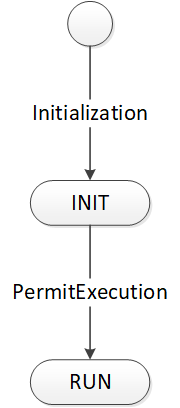
\includegraphics{images/state_diagram}
	\caption{SUM_DIAG state diagram}
\end{figure}

There is no shutdown state, rather DIAG will allow shutdown anytime there are no active diagnostic requests.  An active diagnostic request is defined to be a request ‘Indication’ been received but the corresponding ‘Confirmation’ has not been received.
The SUM_DIAG supports the following UDS services: 
\begin{itemize}
\item DiagnosticSessionControl
\item ECUReset
\item CommunicationControl
\item ReadMemorybyAddress
\item DynamicallyDefineDataIdentifier
\end{itemize}

The RequestHandler service request supplier notification is used to access the above services. It is a runnable that calls the appropriate indication handler.
The following diagram shows the main building blocks of the system.

\begin{figure}[h]
	\centering
		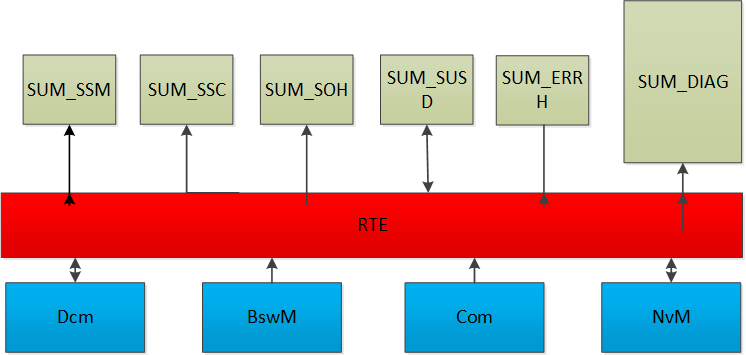
\includegraphics{images/system_block_view}
	\caption{System block view}
\end{figure}

\subsection{SUM_DIAG}

The SUM_DIAG is a software module in the application layer of the standardized architecture of AUTOSAR.  It is primarily intended to be used to implement application level diagnostic functionality such as precondition checks and confirmation for specific diagnostic services.

Due to the configurability required by the DIAG module, the implementation is comprised of static “source” code and generated “source” and “SWCD” files listed below.

Source Files:
\begin{itemize}
\item  SUM_Diag.c
\item  SUM_Diag_Runnables.c
\item  SUM_Diag_Services.c
\item  SUM_DIAG_Ram.c
\item SUM_DIAG_User_file.c
\item SUM_Diag.h
\item SUM_DIAG_Ram.h
\item SUM_DIAG_Types.h
\item SUM_DIAG_User_file.h
\end{itemize}

Generated Files:
\begin{itemize}
\item SUM_Diag_Cfg.c
\item SUM_Diag_Cfg.h
\item SUM_Diag_Cfg_SWCD.arxml
\end{itemize}

\subsection{SUM_SUSD}

A Sender receiver interface is implemented between SUM_SUSD \& SUM_DIAG from which SUM_DIAG receives Permit Execution notification from SUM_SUSD to decide if SUM_DIAG is allowed to execute its functions. SUM_DIAG shall implement the Shutdown Permission interface to SUM_SUSD to indicate whether it has enabled shutdown. 
SUM_DIAG receives also the Vehicle Power Mode in order to observe the driving cycle and possibly updating the MEC value.

\subsection{SUM_SOH}

The Standard Utility Module, State of Health manager (SUM_SOH) contains the following functions: Aggregation/Monitoring of SW platform modes (BSW States), WdgM supervised entity states, reset requests and their occurrences.
When DIAG is requesting an ECU reset or transferring new MEC value, it will notify to 
SUM_SOH.

\subsection{SUM_SSC}

The SUM_SSC module checks all the memory accesses of the UDS services “ReadMemorybyAddress” and “DynamicallyDefineDataIdentifier” and the port to start the SBAT validation to SUM_DIAG. On the other side, SUM_DIAG provides the configured ECU address and MEC value to SUM_SSC.

\subsection{SUM_SSM}

SUM_DIAG provides the notification to SUM_SSM about the status of diagnostics enabling or disabling of normal communications for each channel. In addition, SUM_SSM provides the fault active status and availability notification for the Remote Programming Active Authenticated network signal.

\subsection{Dcm}

The Diagnostics Communication Module (DCM) provides a common API for diagnostic services. The DCM module ensures diagnostic data flow and manages the diagnostic states, especially diagnostic sessions and security state. Furthermore, the DCM module checks if the diagnostic service request is supported and if the service may be executed in the current session according to the diagnostic states.

\subsection{BswM}

SUM_DIAG receives the current communication mode and Diagnostic session from BswM for specific channel. It also gives the communication mode information to SUM_SSM module.

\subsection{NvM}

Non-volatile memory is used to store the Manufacturer Enable Counter Value and the OTA PSF value. SUM_DIAG reads MEC value from NvM to support precondition check needs for diagnostic functions. Moreover, when the OTA PSF changes, SUM_DIAG sends the updated OTA PSF value to the NvM.

\subsection{Com}
The SUM_DIAG module receives from the Com module the Remote Programming Active Authenticated network signal in order to obtain/calculate the OTA PSF value.

\subsection{RTE}

Specifies the system function bus, main communication model etc.

\subsection{SUM\_DIAG\_DcmGetRxPermission callout}

\Requirement{020}
{
The SUM\_DIAG\_DcmGetRxPermission integration callout is invoked by DCM to decide if reception is permitted for a given protocol type and PDU. It takes ProtocolType and DcmRxPduId as inputs and returns E\_OK when protocol, tester source address and vehicle power mode enable conditions are all satisfied; otherwise it returns E\_NOT\_OK. Supported protocol types are limited to the configured pre-emption list (OBDonUDS, OBDS0aD, ZEVonUDS on CAN/ETH) and tester source addresses are restricted to the configured values (for example 0x0E00). The callout shall block pre-emption if the vehicle power mode is OFF or validation fails. 
}
{\Satisfies{SRS_DIAG 122} \Satisfies{SRS_DIAG 123}}

\section{Configuration}

DIAG configuration is done the same way as for standard BSW modules. A parameter definition file is included with the module, which allows the users to configure the available parameters.

\subsection{General Configuration set}
\label{sec:General_Configuration_set}
This section shall describe the General configuration parameters in detail.

\ConfigurationParameter{EcuAddress}
{ECU Address}
{1..1}
{ECUC-INTEGER-PARAM-DEF}
{1..255}
{16}

\ConfigurationParameter{MecInitialValue}
{Manufacturer Enable Counter Initial Value}
{1..1}
{ECUC-INTEGER-PARAM-DEF}
{1..254}
{254}

\Requirement{071}
{
\ConfigurationParameter{PermitExecutionMask}
{PermitExecution mask to start execution of the DIAG module}
{1..1}
{ECUC-INTEGER-PARAM-DEF}
{1..255}
{254}
}{\Satisfies{SRS_DIAG 021}}

\ConfigurationParameter{RMBA_Support}
{RMBA_Support is used to check if ECU supports Read Memory by Address service of DCM}
{1..1}
{ECUC-BOOLEAN-PARAM-DEF}
{NA}
{true}

\ConfigurationParameter{DDDI_Support}
{DDDI_Support is used to check if ECU supports Dynamically Define Data By Memory Address service}
{1..1}
{ECUC-BOOLEAN-PARAM-DEF}
{NA}
{true}

\Requirement{082}
{
\ConfigurationParameter{DiagGenerateInitRunnable}
{This parameter is used to generate a periodic Runnable Entity for calling the DIAG_Init function only once}
{1..1}
{ECUC-BOOLEAN-PARAM-DEF}
{NA}
{false}
}{\Satisfies{SRS_DIAG 106}}

\Requirement{120}
{
\ConfigurationParameter{Sum_Diag_EnableDID_E0CC}
{Sum_Diag_EnableDID_E0CC is used to enable/disable support for DID 0xE0CC (Service Discovery Learning Table Status). When enabled, interfaces and code for DID E0CC are generated. When disabled, SrvcMgr provides an alternative implementation.}
{1..1}
{ECUC-BOOLEAN-PARAM-DEF}
{NA}
{false}
}
{\Satisfies{SRS_DIAG 126} \Satisfies{SRS_DIAG 127}}

\Requirement{109}
{
\ConfigurationParameter{DIAG_TE_Runnable_DIAG_Init_Period}
{This parameter specifies the periodicity, in milliseconds, of the inizialization runnable}
{0..1}
{ECUC-FLOAT-PARAM-DEF}
{1.0..10000.0}
{1000.0}
}{\Satisfies{SRS_DIAG 118}}

\Requirement{110}
{
\ConfigurationParameter{DIAG_TE_Main_Period}
{This parameter specifies the periodicity, in milliseconds, of the main runnable}
{1..1}
{ECUC-FLOAT-PARAM-DEF}
{1.0..10000.0}
{100.0}
}{\Satisfies{SRS_DIAG 118}}

\Requirement{111}
{
\ConfigurationParameter{DIAG_TE_Shutdown_Permission_Period}
{This parameter specifies the periodicity, in milliseconds, of the shutdown permission runnable}
{1..1}
{ECUC-FLOAT-PARAM-DEF}
{1.0..10000.0}
{100.0}
}{\Satisfies{SRS_DIAG 118}}


\Requirement{112}
{
\ConfigurationParameter{DIAG_TE_BswM_ModeUser_Period}
{This parameter specifies the periodicity, in milliseconds, of the Bswm mode runnable}
{1..1}
{ECUC-FLOAT-PARAM-DEF}
{1.0..10000.0}
{100.0}
}{\Satisfies{SRS_DIAG 118}}


\Requirement{113}
{
\ConfigurationParameter{DIAG_TE_MEC_Handler_Period}
{This parameter specifies the periodicity, in milliseconds, of the MEC handler runnable}
{1..1}
{ECUC-FLOAT-PARAM-DEF}
{1.0..10000.0}
{100.0}
}{\Satisfies{SRS_DIAG 118}}

\Requirement{114}
{
\ConfigurationParameter{DIAG_TE_OTA_PSF_Period}
{This parameter specifies the periodicity, in milliseconds, of the OTA PSF runnable}
{1..1}
{ECUC-FLOAT-PARAM-DEF}
{1.0..10000.0}
{100.0}
}{\Satisfies{SRS_DIAG 118}}

\ConfigurationParameter{DIAG_DID_F1A0_MEC_Reference}
{Reference to DCM DID MEC value data}
{1..1}
{ECUC-REFERENCE-DEF}
{NA}
{-}

\ConfigurationParameter{DIAG_DID_F1B0_Reference}
{Reference to DCM DID F1B0 Data}
{0..1}
{ECUC-REFERENCE-DEF}
{NA}
{-}

\Requirement{121}
{
\ConfigurationParameter{DIAG_DID_E0CC_Reference}
{Reference to DCM DID E0CC (Service Discovery Learning Table Status) Data}
{0..1}
{ECUC-REFERENCE-DEF}
{NA}
{-}
}
{\Satisfies{SRS_DIAG 126} \Satisfies{SRS_DIAG 127}}

\ConfigurationParameter{DIAG_MEC_NvMRef}
{Reference to NvM MEC NvMBlockDescriptor}
{1..1}
{ECUC-REFERENCE-DEF}
{NA}
{-}

\ConfigurationParameter{DIAG_OTA_PSF_NvMRef}
{Reference to NvM OTA PSF NvMBlockDescriptor}
{1..1}
{ECUC-REFERENCE-DEF}
{NA}
{-}

\ConfigurationParameter{DIAG_BSPMP_RmtProgmActvAuthRef}
{Reference to the Backup System Power Mode Protected : Remote Programming Active Authenticated signal. This signal can be configured as a single signal or as a signal belonging to a group of signals.}
{1..1}
{ECUC-REFERENCE-DEF}
{NA}
{-}

\ConfigurationParameter{DIAG_ServiceBased_OTA_DataTypeMappingSet}
{Foreign reference to the DATA-TYPE-MAPPING-SET in the system extract used for OTA service-based operations. This parameter references the system data type mapping set that defines the structure and format for OTA service-based functionality and data transformations.}
{0..1}
{ECUC-FOREIGN-REFERENCE-DEF}
{NA}
{-}

\ConfigurationParameter{DIAG_ServiceBased_OTA_Ref}
{Reference to the IMPLEMENTATION-DATA-TYPE for Service Based OTA from System Extract from Software-AR-Packages. This parameter enables OTA service-based operations configuration.}
{0..1}
{ECUC-FOREIGN-REFERENCE-DEF}
{NA}
{-}

\subsection{Config set Configuration}

This section shall describe the Config set container configuration parameters in detail.

\ConfigurationParameter{CommChannels}
{Sub container for communication channels configuratione}
{1..1}
{ECUC-PARAM-CONF-CONTAINER-DEF}
{NA}
{-}

\ConfigurationParameter{CommChannelRef}
{Reference to Communication Channel configuration}
{1..1}
{ECUC-REFERENCE-DEF}
{NA}
{-}
